% Created 2021-03-29 Mon 16:08
% Intended LaTeX compiler: pdflatex
\documentclass[presentation]{beamer}
\usepackage[utf8]{inputenc}
\usepackage[T1]{fontenc}
\usepackage{graphicx}
\usepackage{grffile}
\usepackage{longtable}
\usepackage{wrapfig}
\usepackage{rotating}
\usepackage[normalem]{ulem}
\usepackage{amsmath}
\usepackage{textcomp}
\usepackage{amssymb}
\usepackage{capt-of}
\usepackage{hyperref}
\usetheme{default}
\author{Dinh Duy Kha}
\date{}
\title{Guidelines for Human-AI Tnteraction}
\hypersetup{
 pdfauthor={Dinh Duy Kha},
 pdftitle={Guidelines for Human-AI Tnteraction},
 pdfkeywords={},
 pdfsubject={},
 pdfcreator={Emacs 28.0.50 (Org mode 9.5)}, 
 pdflang={English}}
\begin{document}

\maketitle
\begin{frame}{Outline}
\tableofcontents
\end{frame}


\begin{frame}[label={sec:orga630056}]{Paper: Guidelines for Human-AI interaction}
\begin{itemize}
\item Authors: Saleema Amershi et. al., Microsoft Research
\item Published in: CHI 2018
\end{itemize}
\begin{block}{Overview}
\begin{itemize}
\item 18 design guidelines for human-AI interaction is composed from over 150 design recommendations from over 20 years of learning in AI design
\item The guidelines are validated through multiple rounds user study
\begin{itemize}
\item The results verify he relavant of them and reveals gaps in our knowledge about HAI
\end{itemize}
\end{itemize}
\end{block}
\end{frame}

\begin{frame}[label={sec:org220adea}]{Motivation}
\begin{itemize}
\item \emph{AI-infused systems} ( System that have AI features ) have uncertaintes that violates traditional UI design principles
\item Over 20 years, numerous guidelines and recommendations has been proposed for HAI in the industries and academia
\begin{itemize}
\item However, there are still mistakes made in various AI interfaces
\item Which shows that designers and developers still struggle with creating effective AI-infuse systems
\end{itemize}
\item A shared guidelines is useful for people to design and evaluate AI-infused systems
\end{itemize}
\end{frame}
\begin{frame}[label={sec:org87d86bd}]{Phase 1: Consolidation of guidelines}
\begin{itemize}
\item Guidines are gathered from three sources:
\begin{itemize}
\item Review of industry AI products
\item Recent public articles about AI desgin
\item Relavent papers about AI design
\end{itemize}
\item 168 design guidelines are obtained, which are consolidated into 20
\item The guidelines are organized into four categories based on when during the user's interaction they are applied:
\begin{itemize}
\item Initially
\item During interraction
\item When wrong
\item Over time
\end{itemize}
\end{itemize}
\end{frame}
\begin{frame}[label={sec:orgf0e2743}]{Phase 2: Modified Heuristic Evaluation}
\begin{itemize}
\item 11 team members participated
\item The evaluators examine 13 AI-infused products and try to identify both applications and violations of the guidelines
\item The findings are reviewd, and the number is further reduced to 18
\end{itemize}
\end{frame}
\begin{frame}[label={sec:orgab399d3}]{Phase 3: User study}
\begin{itemize}
\item A user study with 49 HCI particioners is conducted
\end{itemize}
\begin{block}{Procedure}
\begin{itemize}
\item A heuristic evaluation: each participant is asign to an AI product and asked to find applications and violations of each guideline
\end{itemize}
\end{block}
\end{frame}
\begin{frame}[label={sec:org9868d80}]{Phase 3: User study}
\begin{block}{Products}
\begin{itemize}
\item Products are selected using a maximum-variance sampling strategy:
\begin{itemize}
\item Top ranking apps, software and websites in the U.S. is searched
\item Products are grouped by their use case, resulting in 10 categories, 2 product each
\item Select prominent AI-drivent feature to evaluate per product
\end{itemize}
\end{itemize}
\begin{center}
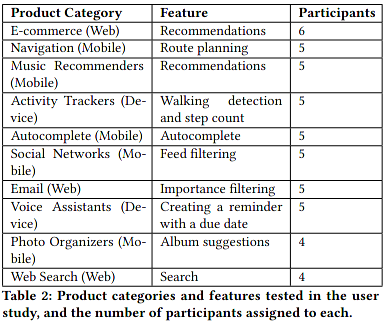
\includegraphics[width=.9\linewidth]{/home/khadd/.dotfiles/dot_doom_d/org/roam/20210328222526-hai_slides.org_20210329_094957_S5Ua6k.png}
\end{center}
\end{block}
\end{frame}
\begin{frame}[label={sec:orgb855954}]{Phase 3: User study}
\begin{block}{Participants}
\begin{itemize}
\item People at large software company with at least 1 year experience in HCI
\item 49 participated
\item 2-3 participants is assigned to each product
\end{itemize}
\end{block}
\begin{block}{Adjustment and Misinterpretaion}
\begin{itemize}
\item The responses are reviewed in the cases of:
\begin{itemize}
\item Duplication (55 instances)
\item The pacipant use ``Does not apply'' to indicate that they cannot find an example of the guideline (73 instances)
\item The pacipant use ``Does not apply'' to indicate a violation (20 instances)
\end{itemize}
+ke clear  The participant misinterpretes one guideline to another
\end{itemize}
\end{block}
\end{frame}
\begin{frame}[label={sec:org21ca6f8}]{Phase 3: User Study (Results)}
\begin{block}{\alert{Clarity and Clarifications}}
\begin{itemize}
\item Some guidelines are rephrased for more clarity
\item Examples:
\begin{itemize}
\item G1: ``Make capabilities clear'' --> ``Make clear \emph{what} the system can do''
\item G2: ``Set expectations of quality'' --> ``Make clear \emph{how well} the system can do what it can do''
\end{itemize}
\end{itemize}
\end{block}
\end{frame}
\begin{frame}[label={sec:orgb053c57}]{Phase 3: User Study (Results)}
\begin{block}{Evolution of guidelines 1 and 2}
\begin{center}
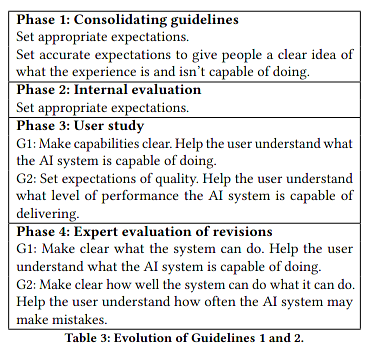
\includegraphics[width=8cm]{/home/khadd/.dotfiles/dot_doom_d/org/roam/20210328222526-hai_slides.org_20210329_145644_YqLBqJ.png}
\end{center}
\end{block}
\end{frame}
\begin{frame}[label={sec:org42abaf0}]{Phase 4: Expert Evaluation}
\begin{itemize}
\item Experts: peoples who have experience in UX/HCI who are familiar with discount usability methods
\item 11 experts are recruited: 6 UX designers, 3 UX researchers, 2 in research and product planning roles
\item Experts are asked to asked to review 9 revised guidelines and chose what they prefer
\begin{center}
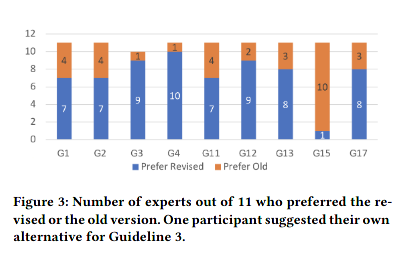
\includegraphics[width=.9\linewidth]{/home/khadd/.dotfiles/dot_doom_d/org/roam/20210328222526-hai_slides.org_20210329_142534_H5hhXl.png}
\end{center}
\end{itemize}

*
\end{frame}

\begin{frame}[label={sec:org42456aa}]{Discussion}
\begin{block}{There is are tradeof between generality and specialization}
\begin{itemize}
\item The guidelines might not be able to address all types of AI-infused system
\begin{itemize}
\item For example, voice-based AI, activity trackers
\end{itemize}
\item Design guidelines that can be easily evaluated from the interface are focused on.
\begin{itemize}
\item Ex: Broarder principles such as ``build trust'' is excluded
\end{itemize}
\end{itemize}
\end{block}
\end{frame}

\begin{frame}[label={sec:org6a9d45f}]{Some guidelines}
\begin{block}{G1: Make clear what the system can do}
\begin{itemize}
\item Help the user understand what the AI system is capable of doing
\item Category: Initially
\item Example: Activity Trackers
\begin{itemize}
\item All metrics that it tracts is displayed and explained how
\end{itemize}
\end{itemize}
\begin{center}
\includegraphics[width=5cm]{/home/khadd/.doom.d/org/.attach/66/5a82cb-2d19-4744-9df1-d92b30a09ab6/_20210329_152534screenshot.png}
\end{center}
\end{block}
\end{frame}
\begin{frame}[label={sec:org62d1e28}]{Some guidelines}
\begin{block}{G4: Show contextually relevant information.}
\begin{itemize}
\item Display information relavent to the user's current task and environment
\item Category: Durring interaction
\item Example: Web Search
\end{itemize}
\begin{center}
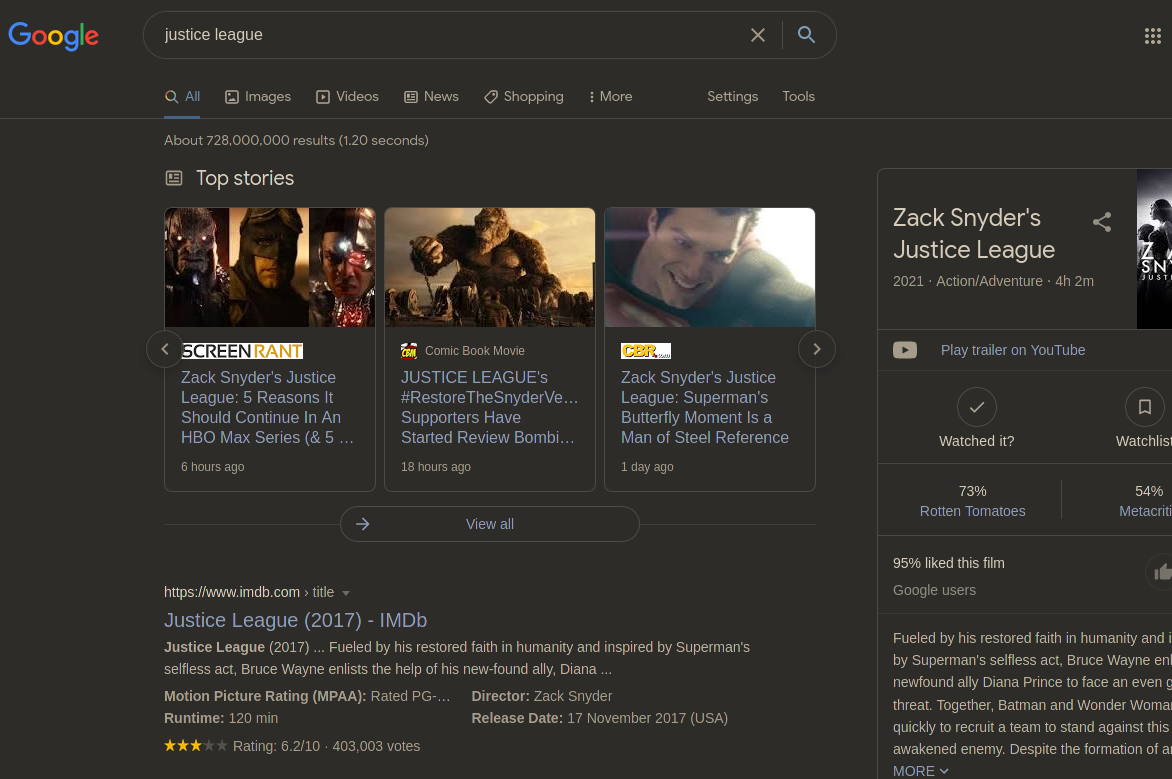
\includegraphics[width=10cm]{/home/khadd/.dotfiles/dot_doom_d/org/roam/20210328222526-hai_slides.org_20210329_153249_iblmLZ.png}
\end{center}
\end{block}
\end{frame}
\begin{frame}[label={sec:orgc303b6a}]{Some guidelines}
\begin{block}{G10: Scope when in doubt.}
\begin{itemize}
\item Engage in disambiguation or gracefully degrade the AI system's services when uncertain about a user's goal
\item Category: When wrong
\item Example: Autocomplete
\begin{itemize}
\item Usually 3-4 suggestion is provided instead of directly completing
\end{itemize}
\end{itemize}
\begin{center}
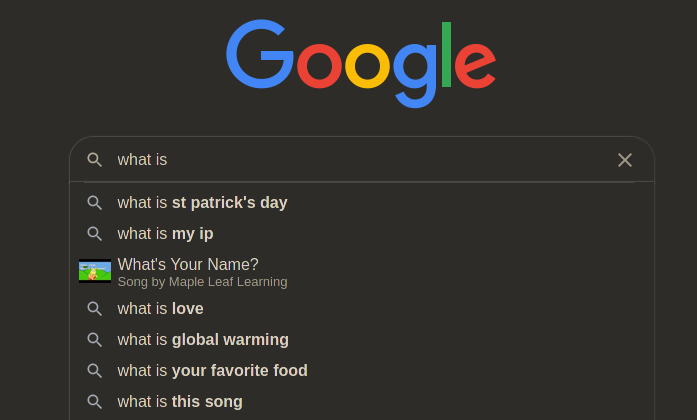
\includegraphics[width=10cm]{/home/khadd/.dotfiles/dot_doom_d/org/roam/20210328222526-hai_slides.org_20210329_153821_U8RpNI.png}
\end{center}
\end{block}
\end{frame}

\begin{frame}[label={sec:org5329745}]{Some guidelines}
\begin{block}{G13: Learn from the user behaviour.}
\begin{itemize}
\item Personalize the user's experience by learning from their actions over time.
\item Category: Overtime
\item Example: Music Recommenders, Video Recommenders
\end{itemize}
\begin{center}
\includegraphics[width=10cm]{/home/khadd/.doom.d/org/.attach/9c/aa3e20-4c07-492c-926a-38e5445e587e/_20210329_154317screenshot.png}
\end{center}
\end{block}
\end{frame}
\end{document}
